\documentclass[a4paper,11pt]{article}
\input{/home/tof/Documents/Cozy/latex-include/preambule_lua.tex}
\newcommand{\showprof}{show them}  % comment this line if you don't want to see todo environment
\fancyhead[L]{La fonction native \emph{sorted}}
\newdate{madate}{10}{09}{2020}
\fancyhead[R]{Terminale - NSI} %\today
\fancyfoot[L]{~\\Christophe Viroulaud}
\fancyfoot[C]{\textbf{Page \thepage}}
\fancyfoot[R]{\includegraphics[width=2cm,align=t]{/home/tof/Documents/Cozy/latex-include/cc.png}}
\usepackage{tikz}

\begin{document}
\begin{Form}
\section{Problématique}
Lors du cours précédent nous sommes revenus sur plusieurs algorithmes de tris étudiés en Première et nous avons étudié leurs performances. Python fournit une fonction native \emph{sorted} et la méthode de liste équivalente \emph{sort}. Nous constatons que cette fonction propose des performances bien meilleures que celles des algorithmes que nous connaissons.
\begin{center}
\shadowbox{\parbox{12cm}{\centering Quel algorithme de tri est implémenté dans la fonction \emph{sorted}?}}
\end{center}
\section{Nouvelle approche}
\subsection{Résoudre des petits problèmes...}
La propriété triviale suivante va nous permettre de construire une nouvelle méthode de tri:
\begin{center}
\guill{Une liste qui contient 0 ou 1 élément est triée.}
\end{center}
\begin{figure}[!h]
\centering
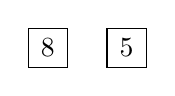
\begin{tikzpicture}[scale=0.5]
\draw (0,0) -- (1,0) ;
\draw (1,0) -- (1,1) ;
\draw (1,1) -- (0,1) ;
\draw (0,1) -- (0,0) ;

\draw (2,0) -- (3,0) ;
\draw (3,0) -- (3,1) ;
\draw (3,1) -- (2,1) ;
\draw (2,1) -- (2,0) ;

\draw (0.5,0.5) node{8};
\draw (2.5,0.5) node{5};
\end{tikzpicture}
\captionof{figure}{Deux listes triées}
\end{figure}
Ainsi deux listes de un élément chacune peuvent être fusionnées en une liste triée de deux éléments.
\begin{figure}[!h]
\centering
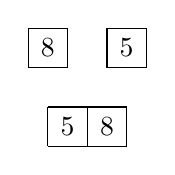
\begin{tikzpicture}[scale=0.5]
\draw (0.5,-1) -- (2.5,-1) ;
\draw (2.5,-1) -- (2.5,-2) ;
\draw (2.5,-2) -- (0.5,-2) ;
\draw (0.5,-2) -- (0.5,-1) ;
\draw (1.5,-1) -- (1.5,-2) ;

\draw (1,-1.5) node{5};
\draw (2,-1.5) node{8};

\draw (0,0) -- (1,0) ;
\draw (1,0) -- (1,1) ;
\draw (1,1) -- (0,1) ;
\draw (0,1) -- (0,0) ;

\draw (2,0) -- (3,0) ;
\draw (3,0) -- (3,1) ;
\draw (3,1) -- (2,1) ;
\draw (2,1) -- (2,0) ;

\draw (0.5,0.5) node{8};
\draw (2.5,0.5) node{5};
\end{tikzpicture}
\captionof{figure}{Fusionner 2 listes de 1 élément}
\end{figure}
\\En résolvant des petits problèmes, nous pouvons remonter à des problèmes plus importants en appliquant le même principe. 
\subsection{...pour solutionner un gros problème}
Essayons de nous ramener à de petits problèmes. Considérons une liste non triée:
\begin{figure}[!h]
\centering
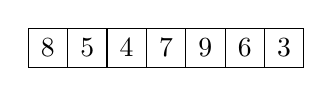
\begin{tikzpicture}[scale=0.5]
\draw (0,0) -- (7,0) ;
\draw (7,0) -- (7,1) ;
\draw (7,1) -- (0,1) ;
\draw (0,1) -- (0,0) ;

\draw (1,0) -- (1,1) ;
\draw (2,0) -- (2,1) ;
\draw (3,0) -- (3,1) ;
\draw (4,0) -- (4,1) ;
\draw (5,0) -- (5,1) ;
\draw (6,0) -- (6,1) ;

\draw (0.5,0.5) node{8};
\draw (1.5,0.5) node{5};
\draw (2.5,0.5) node{4};
\draw (3.5,0.5) node{7};
\draw (4.5,0.5) node{9};
\draw (5.5,0.5) node{6};
\draw (6.5,0.5) node{3};
\end{tikzpicture}
\captionof{figure}{Un gros problème}
\end{figure}
\\Pour se ramener à un problème plus petit, séparons la liste en deux listes:
\begin{figure}[!h]
\centering
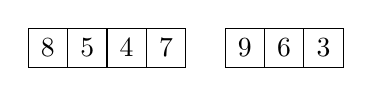
\begin{tikzpicture}[scale=0.5]
\draw (0,0) -- (4,0) ;
\draw (4,0) -- (4,1) ;
\draw (4,1) -- (0,1) ;
\draw (0,1) -- (0,0) ;

\draw (1,0) -- (1,1) ;
\draw (2,0) -- (2,1) ;
\draw (3,0) -- (3,1) ;

\draw (5,0) -- (8,0) ;
\draw (8,0) -- (8,1) ;
\draw (8,1) -- (5,1) ;
\draw (5,1) -- (5,0) ;

\draw (6,0) -- (6,1) ;
\draw (7,0) -- (7,1) ;

\draw (0.5,0.5) node{8};
\draw (1.5,0.5) node{5};
\draw (2.5,0.5) node{4};
\draw (3.5,0.5) node{7};
\draw (5.5,0.5) node{9};
\draw (6.5,0.5) node{6};
\draw (7.5,0.5) node{3};
\end{tikzpicture}
\captionof{figure}{Liste gauche et liste droite}
\end{figure}
\\Il suffit de répéter notre étape de séparation sur les sous-listes engendrées, jusqu'à obtenir des listes de un élément maximum.
\subsection{Diviser pour régner: un algorithme récursif}\label{algo}
Séparer un problème en sous-problèmes se construit très facilement de manière récursive en appelant la fonction de tri sur chaque sous-liste créée.
$$
tri(liste) = \left\{
    \begin{array}{ll}
        liste & \mbox{si la taille de liste} \leq 1 \\
        fusionner(\mbox{tri(liste gauche), tri(liste droite))} & \mbox{sinon }
    \end{array}
\right.
$$
Cet algorithme est celui du \emph{tri fusion}.
\begin{commentprof}
Nous avons déjà utilisé ce type de technique sans le savoir: exponentiation.
\end{commentprof}
\subsection{L'étape de fusion}
Il est aisé de construire une liste triée à partir de deux listes déjà triées. Il suffit de prendre le plus petits éléments parmi nos deux listes et l'ajouter à la liste finale, et ce jusqu'à épuisement des listes.
\begin{activite}
Écrire une fonction \textbf{fusionner(gauche: list, droite: list)\;\rightarrow\;list} qui renvoie une liste triée composée des éléments de \emph{gauche} et \emph{droite} déjà triées.
\end{activite}
\subsection{Le code complet du tri fusion}
\begin{activite}
En s'appuyant sur la description récursive de l'algorithme au paragraphe \ref{algo}, écrire une fonction \textbf{tri\_fusion(l: list)\;\rightarrow\;list} qui renvoie la liste \emph{l} triée.
\end{activite}
\section{Performances du tri fusion}
\subsection{Comparaison}
\begin{activite}
\begin{enumerate}
\item Créer un tuple \emph{l} de 10000 entiers compris entre 0 et 1000.
\item En utilisant la fonction (\emph{duree\_tri}) créée précédemment, effectuer une mesure de la durée d'exécution du tri fusion sur une liste dérivant du tuple l.
\item Effectuer la même mesure avec la fonction \emph{sorted}.
\item Proposer plusieurs explications quant à la différence constatée.
\end{enumerate}
\end{activite}
\begin{commentprof}
La fonction \emph{fusionner} n'est pas optimisée: elle utilise pop(0) qui reconstruit une liste à chaque fois.\\
tri\_fusion copie également des listes\\
langage C
\end{commentprof}
\subsection{Complexité}
\subsubsection{Découper en sous-listes}
À chaque appel de la fonction \emph{tri\_fusion} nous divisons la liste en deux. La question à se poser est de savoir combien de fois faut-il couper la liste en deux pour obtenir des listes de un élément. Mathématiquement nous cherchons \emph{a} tel que: $$\dfrac{n}{2^a}=1$$
Le logarithme base 2 noté $log_2$ se définit: $log_2(2^x)=x$.
\begin{activite}
Déterminer la valeur de \emph{a} en fonction de \emph{n}.
\end{activite}
\begin{commentprof}
La complexité de la fonction \emph{tri\_fusion} est en $O(log_2(n))$. Et on ne peut pas faire mieux!
\end{commentprof}
\subsubsection{Fusionner deux listes}
La fonction \emph{fusionner} réalise \emph{n} comparaisons pour assembler deux listes de taille $\dfrac{n}{2}$.
\begin{figure}[!h]
\centering
\begin{tikzpicture}[scale=0.45]
\draw (0,1) circle(1);
\draw (-6,-2) circle(1);
\draw (6,-2) circle(1);
\draw (-8,-5) circle(1);
\draw (-4,-5) circle(1);
\draw (4,-5) circle(1);
\draw (8,-5) circle(1);
\draw (-9,-8) circle(1);
\draw (-7,-8) circle(1);
\draw (-5,-8) circle(1);
\draw (-3,-8) circle(1);
\draw (3,-8) circle(1);
\draw (5,-8) circle(1);
\draw (7,-8) circle(1);
\draw (9,-8) circle(1);

\draw (-10,-12) circle(1);
\draw (-8,-12) circle(1);
\draw (-6,-12) circle(1);
\draw (-4,-12) circle(1);
\draw (-2,-12) circle(1);
\draw (0,-12) circle(1);
\draw (2,-12) circle(1);
\draw (4,-12) circle(1);
\draw (6,-12) circle(1);
\draw (8,-12) circle(1);
\draw (10,-12) circle(1);

\draw (0,0) -- (-6,-1) ;
\draw (0,0) -- (6,-1) ;
\draw (-6,-3) -- (-8,-4) ;
\draw (-6,-3) -- (-4,-4) ;
\draw (6,-3) -- (8,-4) ;
\draw (6,-3) -- (4,-4) ;
\draw (-8,-6) -- (-9,-7) ;
\draw (-8,-6) -- (-7,-7) ;
\draw (-4,-6) -- (-5,-7) ;
\draw (-4,-6) -- (-3,-7) ;
\draw (8,-6) -- (9,-7) ;
\draw (8,-6) -- (7,-7) ;
\draw (4,-6) -- (5,-7) ;
\draw (4,-6) -- (3,-7) ;

\draw (0,1) node{$n$};
\draw (-6,-2) node{$\dfrac{n}{2}$};
\draw (6,-2) node{$\dfrac{n}{2}$};
\draw (-8,-5) node{$\dfrac{n}{4}$};
\draw (-4,-5) node{$\dfrac{n}{4}$};
\draw (4,-5) node{$\dfrac{n}{4}$};
\draw (8,-5) node{$\dfrac{n}{4}$};
\draw (-9,-8) node{$\dfrac{n}{8}$};
\draw (-7,-8) node{$\dfrac{n}{8}$};
\draw (-5,-8) node{$\dfrac{n}{8}$};
\draw (-3,-8) node{$\dfrac{n}{8}$};
\draw (3,-8) node{$\dfrac{n}{8}$};
\draw (5,-8) node{$\dfrac{n}{8}$};
\draw (7,-8) node{$\dfrac{n}{8}$};
\draw (9,-8) node{$\dfrac{n}{8}$};
\draw (0,-10) node{.........};

\draw (-10,-12) node{$1$};
\draw (-8,-12) node{$1$};
\draw (-6,-12) node{$1$};
\draw (-4,-12) node{$1$};
\draw (-2,-12) node{$1$};
\draw (0,-12) node{$1$};
\draw (2,-12) node{$1$};
\draw (4,-12) node{$1$};
\draw (6,-12) node{$1$};
\draw (8,-12) node{$1$};
\draw (10,-12) node{$1$};

\draw (18,1) node{$n$};
\draw (18,-2) node{$2×(\dfrac{n}{2})=n$};
\draw (18,-5) node{$2^2×(\dfrac{n}{2^2})=n$};
\draw (18,-8) node{$2^3×(\dfrac{n}{2^3})=n$};
\draw (18,-12) node{$2^{log_2(n)}×(\dfrac{n}{2^{log_2(n)}})=n$};

\end{tikzpicture}
\captionof{figure}{Nombre de comparaisons}
\end{figure}
\subsubsection{Complexité du tri fusion}
Chaque niveau de fusion a un coup de \emph{n} et il y a $log_2(n)$ niveaux.
\begin{center}
\shadowbox{\parbox{10cm}{\centering La complexité du tri fusion est en $O(n×log_2(n))$.}}
\end{center}
\subsection{Stabilité}
On dit qu'un algorithme de tri est stable s'il ne modifie pas l'ordre initial des clés identiques.
\begin{activite}
\begin{enumerate}
\item À la main sur quelques exemples, vérifier si le tris par sélection et par insertion sont stables.
\item Vérifier la stabilité du tri fusion.
\end{enumerate}
\end{activite}
\section{La fonction native \emph{sorted}}
Elle implémente l'algorithme \emph{Timsort} mis au point par Tim Peters en 2002. C'est un algorithme hybride de plusieurs tris.
\begin{activite}
Réaliser une présentation de l'algorithme \emph{Timsort}. Il n'est pas demandé d'effectuer une étude théorique précise mais d'expliquer le fonctionnement général et les choix de Tim Peters.
\end{activite}
\end{Form}
\end{document}